\documentclass[10pt,letterpaper]{article}

% Packages
\usepackage[utf8]{inputenc}
\usepackage[top=0.85in,left=1.5in,footskip=0.75in]{geometry}
\usepackage{lastpage,fancyhdr,graphicx}
\usepackage{epstopdf}
\usepackage{verbatim}
\usepackage{amsmath}
\usepackage{amsfonts}
\usepackage{hyperref}
\usepackage{setspace}

% Text layout
\raggedright
\setlength{\parindent}{0.5cm}
\textwidth 5.5in 
\textheight 8.75in
\onehalfspacing

% Bibliography
\usepackage[backend=biber,style=numeric,sorting=ynt]{biblatex}
\addbibresource{bibliography.bib}

% C++ symbol
\newcommand{\CC}{C\nolinebreak\hspace{-.05em}\raisebox{.4ex}{\tiny\bf +}\nolinebreak\hspace{-.10em}\raisebox{.4ex}{\tiny\bf +}}
\def\CC{{C\nolinebreak[4]\hspace{-.05em}\raisebox{.4ex}{\tiny\bf ++}}}

% Header and footer
\pagestyle{fancy}
\fancyhf{}
\rfoot{\thepage/\pageref{LastPage}}
\renewcommand{\headrulewidth}{0pt}
\fancyheadoffset[L]{2.25in}
\fancyfootoffset[L]{2.25in}

\begin{document}

\vspace*{0.2in}

\begin{centering}
{\huge\textbf\newline{Pandemia: Overview}}
\\
\bigskip

\includegraphics[width=0.2\textwidth]{pandemia_logo}
\\
\bigskip
\today
\\
\end{centering}

\subsection*{Introduction}
Pandemia is an individual-based stochastic pandemic model, able to simulate the spread of an infectious disease over multiple regions, including the entire world. The model is fast and scalable, able to simulate extremely large numbers of individuals. This document presents an overview of the model.

\subsection*{World}
The Pandemia model acts on a \textbf{World}, with each \textbf{World} consisting of \textbf{Regions}, with each \textbf{Region} consisting of \textbf{Agents}, \textbf{Locations} and \textbf{Activities}. Each agent performs a sequence of activities and performs these activities at particular locations. For a world $W$ containing a region $R$, let us denote by $I$, $L$ and $A$ the sets of agents, locations and activities associated to region $R$. Then, denoting by $T$ the time index set, to each agent $i \in I$ is associated a sequence of activities $$\alpha_i : T \rightarrow A$$ and a random variable $$\lambda_i : A \times \Omega \rightarrow L$$ determining the location $\lambda_i(a_i(t),\omega)$ of agent $i$ at time $t$. A \textbf{World} additionally consists of a \textbf{Travel Matrix}, representing how many agents travel from each region to each other region each day. Here is the simplest possible \textbf{World} structure:
\begin{itemize}
\item One \textbf{Region}, one \textbf{Activity}, one \textbf{Location} and any number of \textbf{Agents}.
\end{itemize}
Here is the most complicated:
\begin{itemize}
\item Several \textbf{Regions}, with each \textbf{Region} consisting of several \textbf{Activities}, any number of \textbf{Locations} and any number of \textbf{Agents}, with a \textbf{Travel Matrix} describing the mixing between regions.
\end{itemize}
The \textbf{World} object, having been built, can be saved and thus it is not necessary to complete the build phase each time a simulation is run. The \textbf{World} object is fed into the simulator.

\subsection*{Components}
The model features of a number of components, most of which are optional:
\begin{itemize}
\item \textbf{Movement}
\item \textbf{Travel}
\item \textbf{Health}
\item \textbf{Hospitalization}
\item \textbf{Testing and Contact Tracing}
\item \textbf{Vaccination}
\item \textbf{Seasonality}
\end{itemize}
Additional or alternative components are easily added. Pandemia provides a default model for each component. The details of these default models are described in separate documents. The main Pandemia loop looks approximately as follows:
\begin{center}
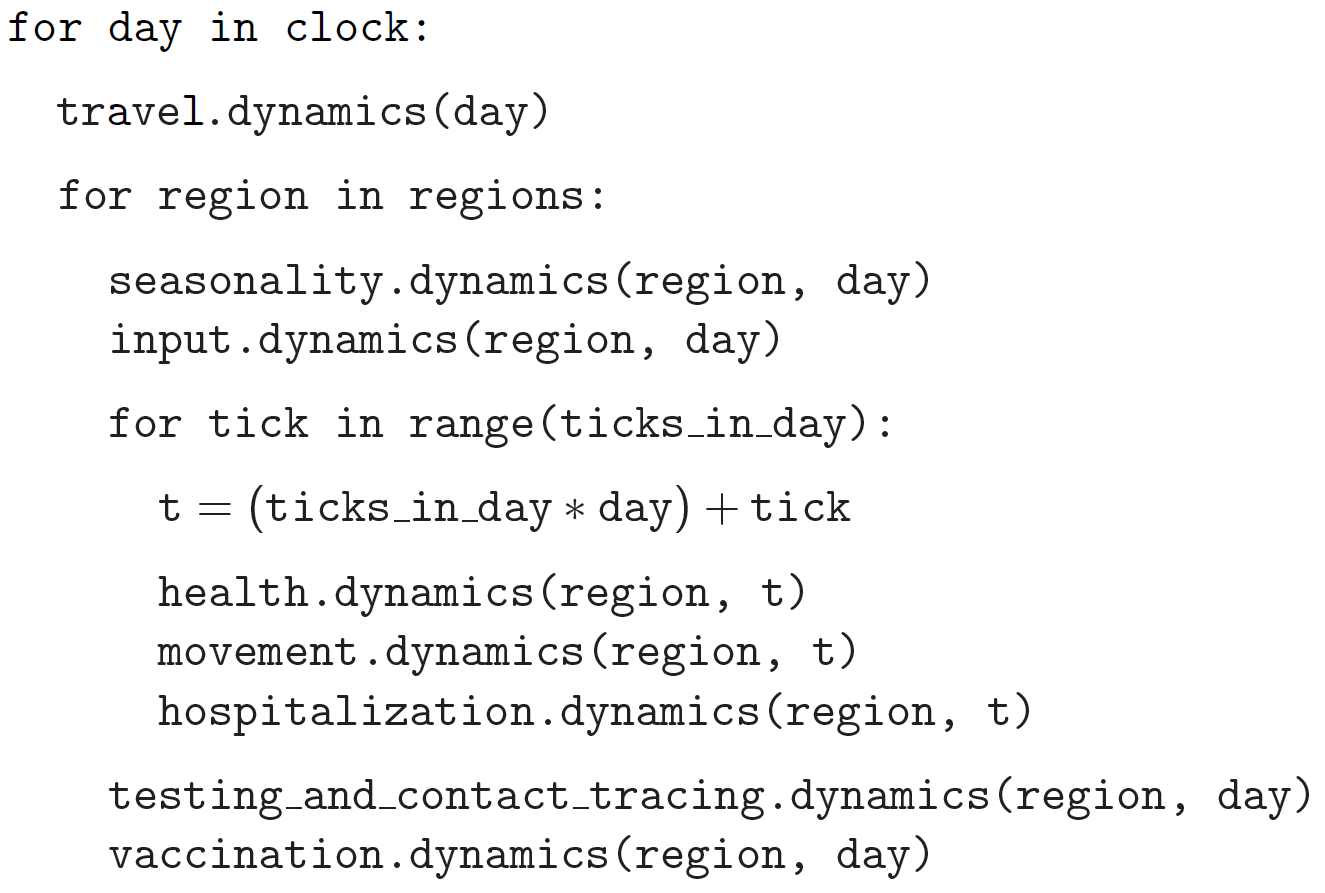
\includegraphics[width=0.65\textwidth]{psuedo}
\end{center}
Note that some components update each day, while others update each tick. At the beginning of each day, Pandemia decides who is travelling from each region to each other region, and infects these travellers based on the average infectiousness of their destination region. These travellers are then set aside for the remainder of the day. Pandemia then loops over all the regions, performing independent individual-based simulations on a finer timescale. Since these simulations are independent, the loop over the regions can be parallelized. In this way, Pandemia is both fast and scalable. Even on a laptop computer, using 15 CPUs and 24GB of RAM, it has been able to perform a 100 day simulation, with a 1 hour tick length, of over 100 million individuals, in under 1.5 hours.

\pagebreak

\subsection*{Interventions}
The \textbf{Input} component allows the user to specify a \textbf{Policy}, consisting of interventions. Possible interventions include the following:
\begin{itemize}
\item \textbf{Lockdown}
\item \textbf{Border Closure}
\item \textbf{Vaccination}
\item \textbf{Testing and Contact Tracing}
\item \textbf{Quarantine}
\item \textbf{Face Masks}
\end{itemize}
Additional or alternative interventions are easily added. \textbf{Reporters} collect output data for visualization and analysis.

\end{document}